\documentclass{article}

\usepackage{listings}
\usepackage{float}
\usepackage{xcolor}
\usepackage{mathtools}
\lstset{
    language=Matlab,                % 设置语言为MATLAB
    basicstyle=\ttfamily\footnotesize, % 使用等宽字体,稍小一点的尺寸
    keywordstyle=\bfseries\color{blue!70!black}, % 关键字加粗并设置为深蓝色
    commentstyle=\itshape\color{green!50!black}, % 注释使用斜体,深绿色
    stringstyle=\color{orange},     % 字符串设置为橙色
    numbers=left,                   % 在左侧显示行号
    numberstyle=\tiny\color{gray},  % 行号样式:小号灰色字体
    stepnumber=1,                   % 每行都显示行号
    numbersep=5pt,                  % 行号与代码之间的间距
    backgroundcolor=\color{white},  % 背景颜色为白色
    showspaces=false,               % 不显示空格标记
    showstringspaces=false,         % 不显示字符串中的空格
    showtabs=false,                 % 不显示制表符
    frame=single,                   % 单线边框
    rulecolor=\color{lightgray},    % 边框颜色为浅灰色
    tabsize=4,                      % 制表符大小为4个空格
    captionpos=b,                   % 标题位置在底部
    breaklines=true,                % 自动换行
    breakatwhitespace=true,         % 只在空格处断行
    title=\lstname,                 % 显示文件名作为标题
    escapeinside={\%*}{*)},         % 允许在代码中添加LaTeX注释
    morekeywords={*}                % 可以添加额外的MATLAB关键字
}
\usepackage[UTF8]{ctex}
\usepackage{graphicx}
\usepackage[colorlinks=true, allcolors=blue]{hyperref}

\title{matlab光谱频率分析报告}
\author{伍紫涵 \ 芦炳诚}
\date{2025/08/31}

\begin{document}
\maketitle

\pagenumbering{roman}
\tableofcontents
\newpage
\pagenumbering{arabic}
\section{Object of the Practical}
In this lecture, we will use mainly Matlab for the illustrations. The main objectives are

1) Familiar with some related scientific English words (vocabulary);

2) Able to efficiently use Matlab;

3) Get some knowledges of the typical applications of estimating frequencies in a signal;

4) Understand some classical non parametric frequency estimation methods;

5) Understand some typical parametric high resolution methods;

6) Understand and able to program some spectral analysis techniques with Matlab.
\section{Learning MatLab}
\subsection{Question 1}

%question 1
\begin{lstlisting}
v = 1: 100

w = -cos(v * pi)
\end{lstlisting}
\begin{figure}[H]
    \centering
    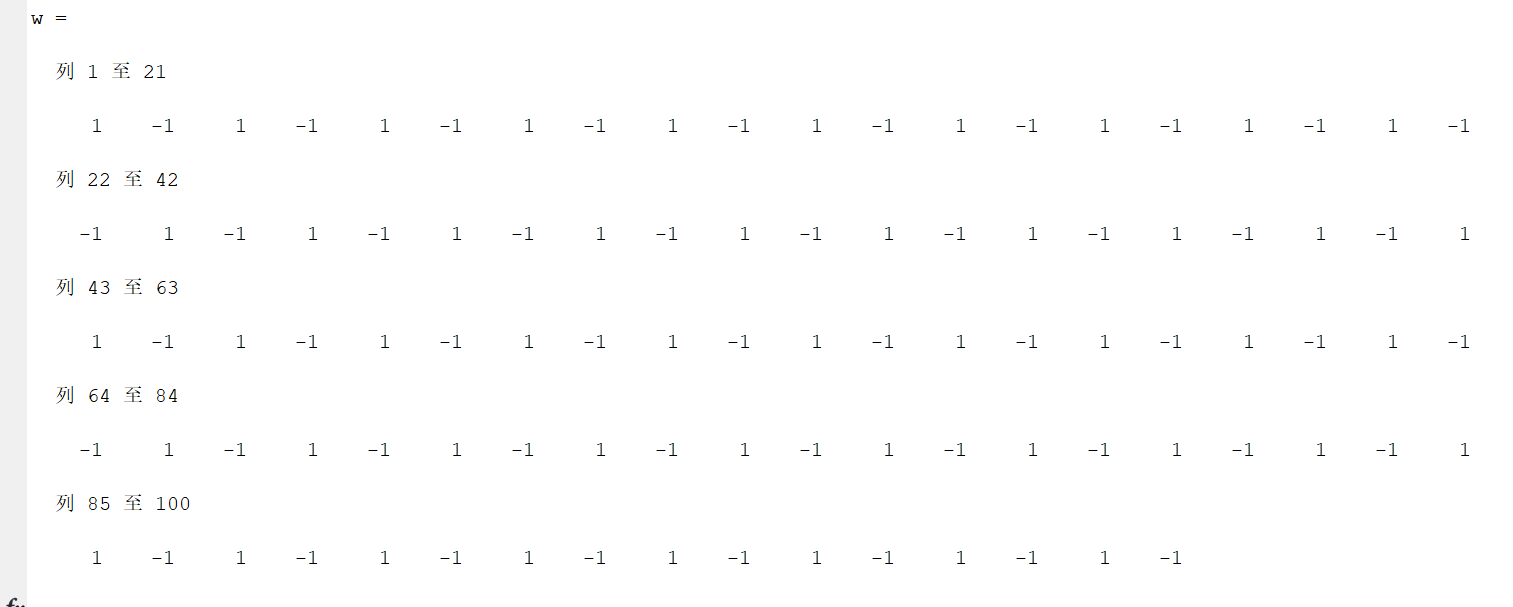
\includegraphics[width=1\linewidth]{0c2363eb7126e75d7f1f5923d619db77.png}
    \caption{result 1}
    \label{fig:1}
\end{figure}

\subsection{Question 2}
\begin{lstlisting}
a = zeros(1, 200)

a(1:2:end) = 1:100
\end{lstlisting}
\begin{figure}[H]
    \centering
    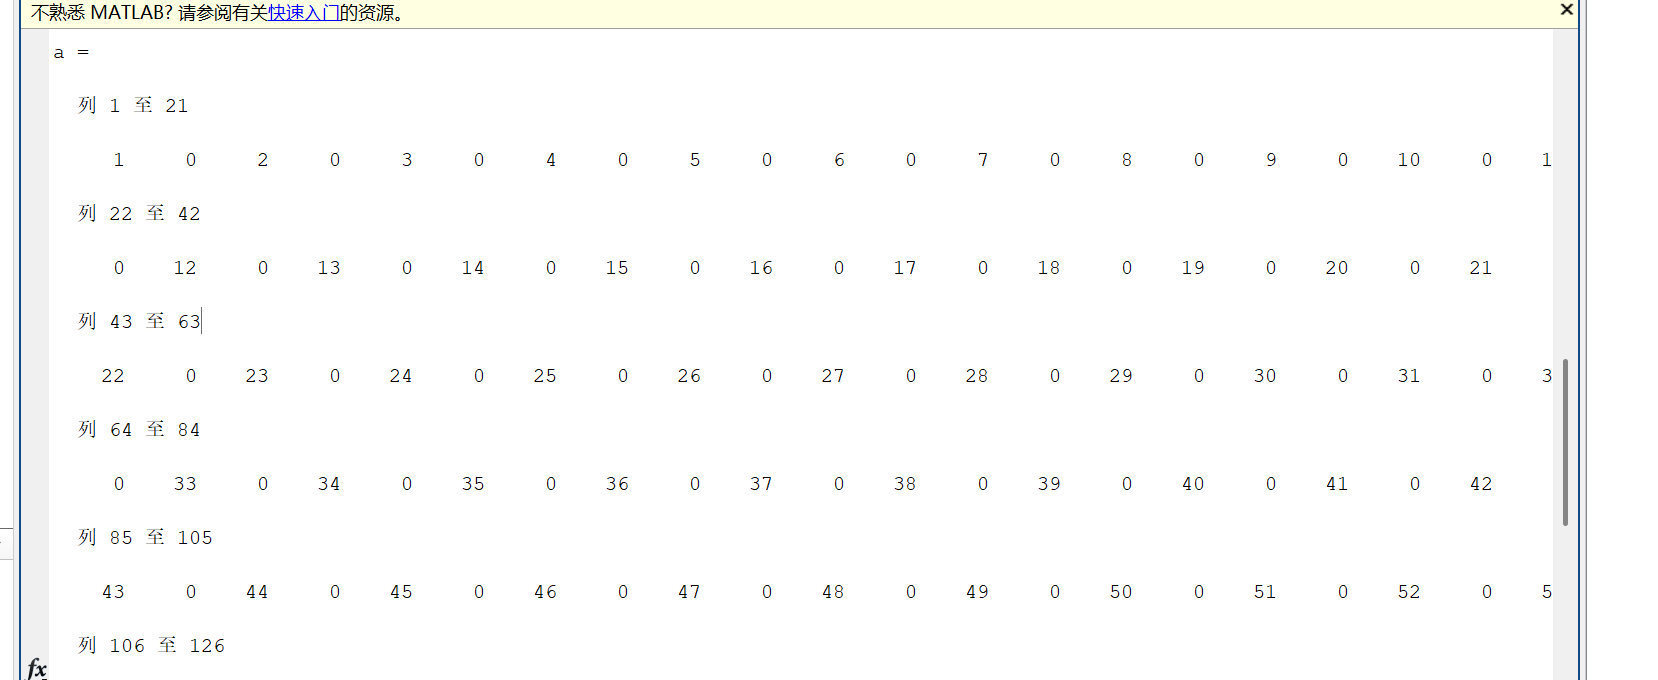
\includegraphics[width=1\linewidth]{2.png}
    \caption{result 2}
    \label{fig:2}
\end{figure}

\subsection{Question 3}
\begin{lstlisting}
A = [75, 80, 90; 50, 75, 55; 65, 80, 50]

coefficient = [3; 2; 1]

B = A * coefficient / sum(coefficient)
\end{lstlisting}
\begin{figure}[H]
    \centering
    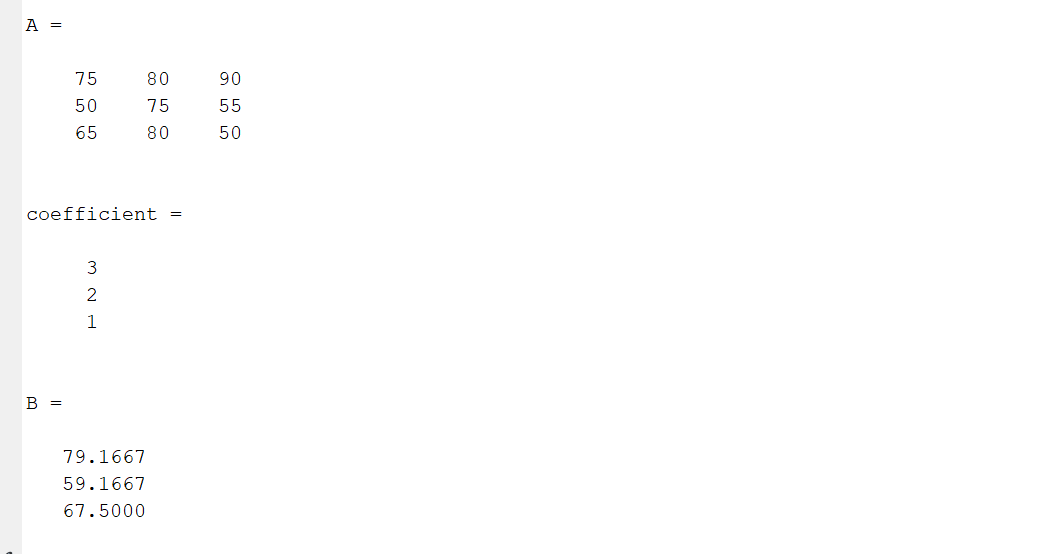
\includegraphics[width=1\linewidth]{3.png}
    \caption{result 3}
    \label{fig:3}
\end{figure}

\subsection{question 4}
\begin{lstlisting}
C = 1:10

D = repmat(C,3,1)
\end{lstlisting}
\begin{figure}[H]
    \centering
    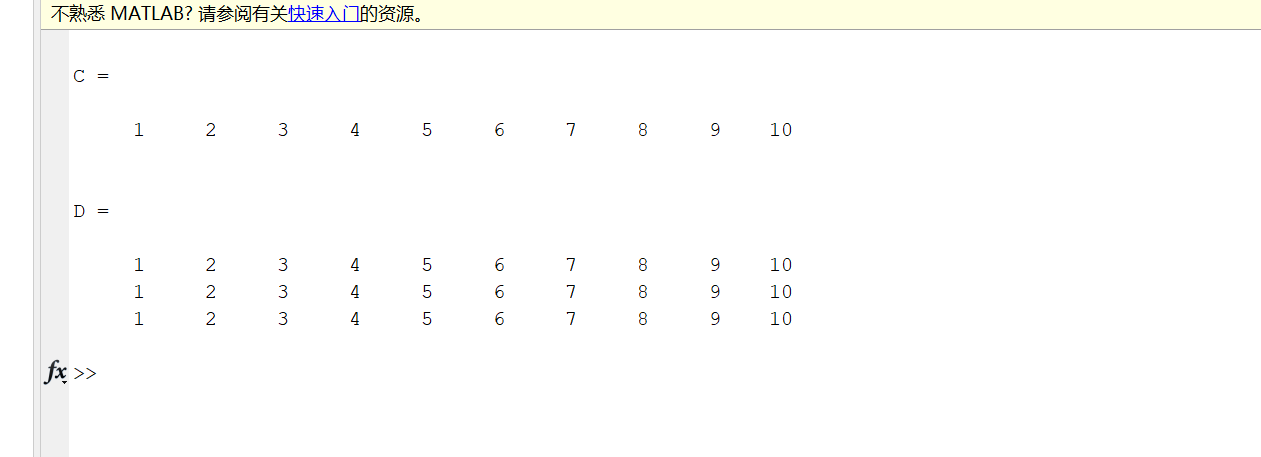
\includegraphics[width=1\linewidth]{4.png}
    \caption{result 4}
    \label{fig:4}
\end{figure}

\subsection{question 5}
\begin{lstlisting}
E = [1, 2; 3, 4]

F = [1;3]

ans = inv(E) * F
\end{lstlisting}
\begin{figure}[H]
    \centering
    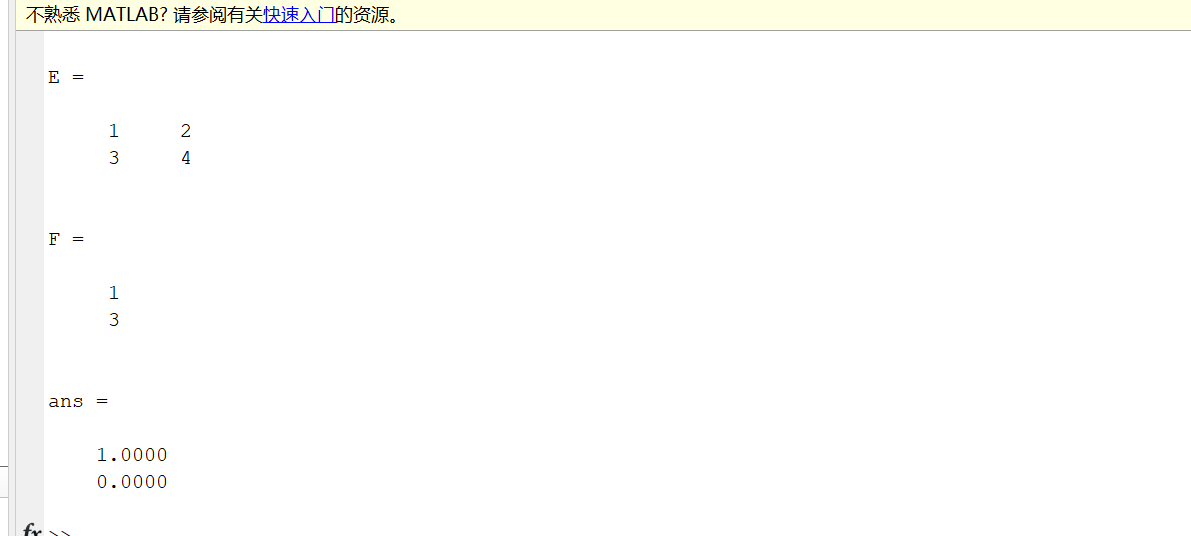
\includegraphics[width=1\linewidth]{5.png}
    \caption{Enter Caption}
    \label{fig:5}
\end{figure}

\subsection{question 6}
\begin{lstlisting}
A = 1;

f0 = 1;

t = (1:0.001:10);

x = A * cos(2 * pi * f0 * t);

plot(t, x)

title ('cos signal with frequency 1Hz')

xlabel('time in second')

ylabel('amplitue')

\end{lstlisting}
\begin{figure}[H]
    \centering
    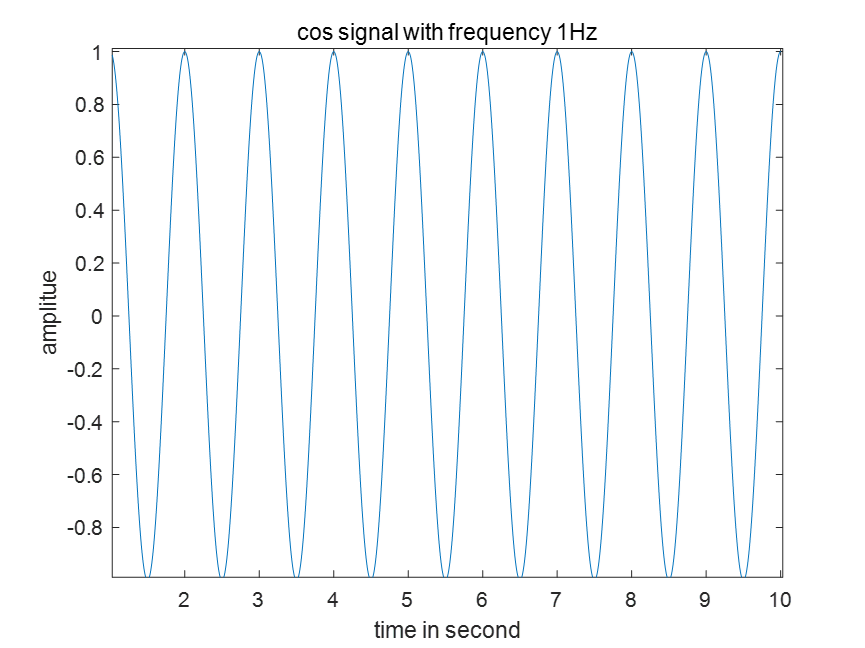
\includegraphics[width=1\linewidth]{6.png}
    \caption{result 6}
    \label{fig:6}
\end{figure}

\subsection{question 7}
\begin{lstlisting}
A = 1;

f0 = 1;

t = (1:0.001:10);

subplot(2, 1, 1)

x = A * cos(2 * pi * f0 * t);

plot(t, x)

title ('cos signal with frequency 1Hz')

xlabel('time in second')

ylabel('amplitue')

f0 = 2;

subplot(2, 1, 2)

x = A * cos(2 * pi * f0 * t);

plot(t, x)

title ('cos signal with frequency 2Hz')

xlabel('time in second')

ylabel('amplitue')
\end{lstlisting}
\begin{figure}[H]
    \centering
    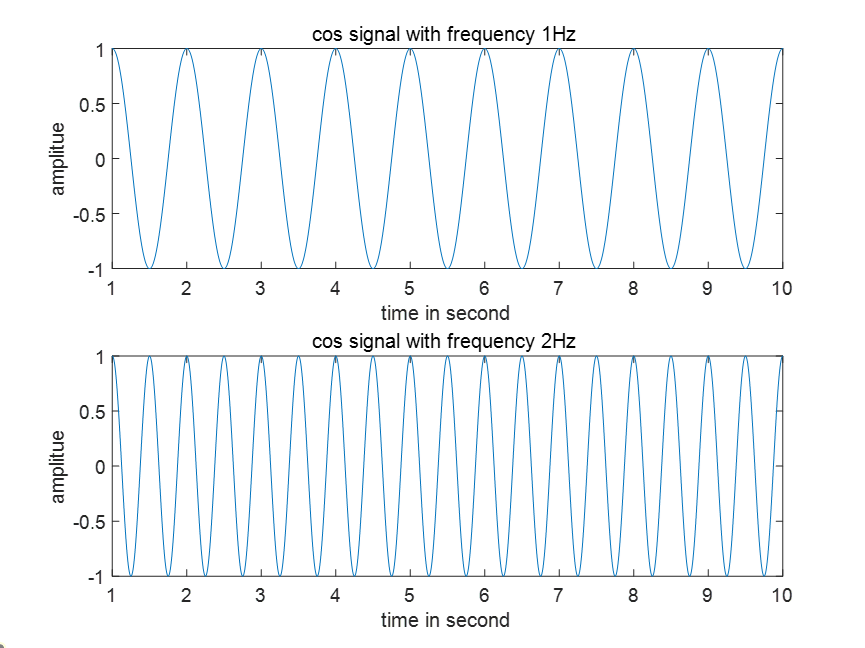
\includegraphics[width=1\linewidth]{7.png}
    \caption{Enter Caption}
    \label{fig:7}
\end{figure}
\subsection{question 8}
\begin{lstlisting}
A = 1;

t = (1:0.001:10);

x = A * cos(2 * pi * 1 * t);

y = A * cos(2 * pi * 2 * t);

plot(t, x)

hold on

plot(t, y)

title ('cos signal with frequency 1/2Hz')

xlabel('time in second')

ylabel('amplitue')

\end{lstlisting}
\begin{figure}[H]
    \centering
    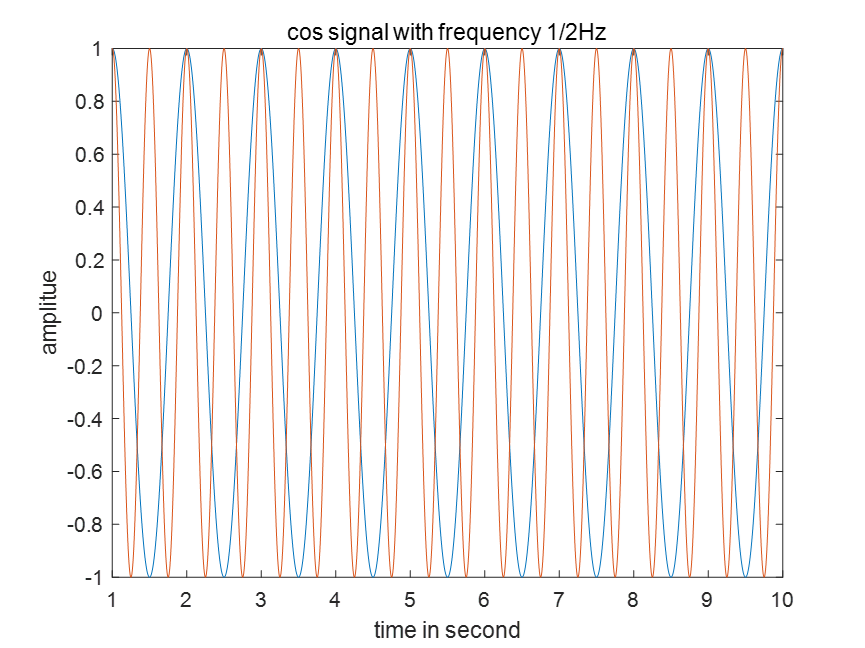
\includegraphics[width=1\linewidth]{8.png}
    \caption{Enter Caption}
    \label{fig:8}
\end{figure}

\section{Work Theoretical Preparation}
Consider a continuous-time signal $x(t)$ with spectrum $X(f)$. We sample $x(t)$ with sampling frequency $f_s = \frac{1}{T_s}$ to get samples $x(nT_s)$. We want to estimate the spectrum of this signal with a DFT (Discrete Fourier transform) of order $N_f$.

1. Write the Fourier transform $X(f)$ of $x(t)$.

\begin{equation}
    X(f) = \int_{-\infty}^{+\infty}x(t)e^{-j2\pi ft}\,dt
\end{equation}

2. Write the Fourier transform $X_s(f)$ of $x(nT_s)$.

\begin{equation}
    X_s(f) = FT(x(nT_s)) = \sum_{n=-\infty}^{+\infty} x(nT_s)e^{-j2\pi fnT_s}
\end{equation}

3. What are the main properties of $X_s(f)$? Give the relationship of $X_s(f)$ in terms of $X(f)$.

\begin{equation}
    X_s(f+f_s) = X_s(f) = \frac{1}{T_s} \sum_{k=-\infty}^{+\infty}X(f-\frac{k}{T_s})
\end{equation}

In practice we can get only a limited number of samples of $x(nT_s)$, for $n = 0,1,\ldots,N_t-1$. Mathematically, it is equivalent to multiply $x(nT_s)$ by the following rectangular window:

\[
w(nT_s) =
\begin{dcases}
    1 & n = 0,1,\ldots,N_t-1\\
    0 & \text{otherwise}
\end{dcases}
\]

Then the observed signal can be written as 

\[
y(nT_S)=
\begin{dcases}
    x(nT_S) & n = 0,1,\ldots,N_t-1\\
    0 & \text{otherwise}
\end{dcases}
\]

4. Calculate mathematically the Fourier transform $W_s(f)$ of $w(nT_s)$.

\begin{equation}
    w(nT_s) =
    \begin{dcases}
        1 & 0 \leq n \leq N_t-1\\
        0 & \text{if not}
    \end{dcases}
\end{equation}

\begin{equation}
    W_s(f) 
    = \sum_{n=-\infty}^{+\infty}w_s(nT_s)e^{-j2\pi fnT_s}
    = \sum_{n=0}^{N_t-1}e^{-j2\pi fnT_s}
    = \frac{1-e^{-j2\pi fN_tT_s}}{1-e^{-j2\pi fT_s}}
    = e^{-j\pi f(N_t-1)T_s}\frac{sin(\pi fN_tT_s)}{sin(\pi fT_s)}
\end{equation}

5. For which frequencies, $W_s(f)$ is zero ?

\begin{equation}
    W_s(f) = 0 => sin(\pi fN_tT_s)=0 => \pi fN_tT_s=k\pi => f=\frac{k}{N_tT_s}
\end{equation}

6. What is the width of the mainlobe of the above spectrum ? 

\begin{equation}
    mainlobe~width = \frac{2}{N_tT_s}
\end{equation}

7. Write the expression of the Fourier transform $(FT)Y_S(f)$ of $y(nT_s)$.

\begin{equation}
    Y_s(f) = \sum_{n=0}^{N_t-1}y(nT_s)e^{-j2\pi fnT_s}
\end{equation}

8. Write the discrete Fourier transform of $y(nT_s)$, of order $N_f$.

\begin{equation}
    Y_k = \sum_{n=0}^{N_t-1}y(nT_s)e^{-j2\pi \frac{k}{N_f}n}
\end{equation}

9. The DFT of order $N_f$ evaluates the spectrum $Y_s(f)$ for how many frequencies? Specify them.

DFT assess $Y_s(f)$ for N_f points specified by $\frac{k}{N_fT_s}$, k=0,1,2,\ldots,N_f-1

10. Among all the above frequencies, what is the difference between two successive frequencies (precision of DFT)? 

\begin{equation}
    \triangle f = \frac{1}{N_fT_s}
\end{equation}

11. What is the spectrum of $e^{j2\pi f_0nT_s}w(nT_s)$ ?

\begin{equation}
    TF[e^{j2\pi f_0nT_sw(nT_s)}w(nT_s)] = W(f-f_0)
\end{equation}

12. What is the spectrum of $cos(2\pi f_0nT_s)w(nT_s)$ ?

\begin{equation}
    TF[cos(2\pi f_0nT_s)w(nT_s)] = \frac{1}{2}W(f-f_0) + \frac{1}{2}W(f+f_0)
\end{equation}

\section{Description and Result Explaination}
\subsection{Result}
\begin{lstlisting}
    close all;
 clear all;
 clc;
 F1=10;
 Fs=8;
 Ts=1/Fs;
 Nt=32;
 t=(0:(Nt-1))*Ts;
 x=cos(2*pi*F1*t);
 y32=abs(fft(x,32))/Nt;
 y64=abs(fft(x,64))/Nt;
 y128=abs(fft(x,128))/Nt;
 y1024=abs(fft(x,1024))/Nt;

 subplot(3,2,1)
 t1=0:Ts/100:(Nt-1)*Ts;
 y1=cos(2*pi*F1*t1);
 plot(t1,y1);
 hold on
 plot(t,x,'O')
 xlabel('time')

 subplot(3,2,2)
 faxe=((0:32-1)/32)*Fs;
 stem(faxe,y32,'.')     %修改,显示全部的频谱而不截取,从而看到双峰
 xlabel('frequency Nf=32')

 subplot(3,2,3)
 faxe=((0:64-1)/64)*Fs;
 %plot(faxe,y64,'.')
 stem(faxe,y64,'.')     %同上
 xlabel('frequency Nf=64')
 faxe=((0:128-1)/128)*Fs;

 subplot(3,2,4)
 stem(faxe,y128,'.')    %同上
 %stem(faxe,y128)
 xlabel('frequency Nf=128')

 faxe=((0:1024-1)/1024)*Fs;
 subplot(3,2,5)
 plot(faxe,y1024,'.')   %同上
 %stem(faxe,y128)
 xlabel('frequency Nf=1024')
 faxe=((0:1024-1)/1024)*Fs;
 subplot(3,2,6)
 plot(faxe,y1024)       %同上
 %stem(faxe,y128)
 xlabel('frequency Nf=1024')
\end{lstlisting}

图片展示如下:
\begin{figure}[H]
    \centering
    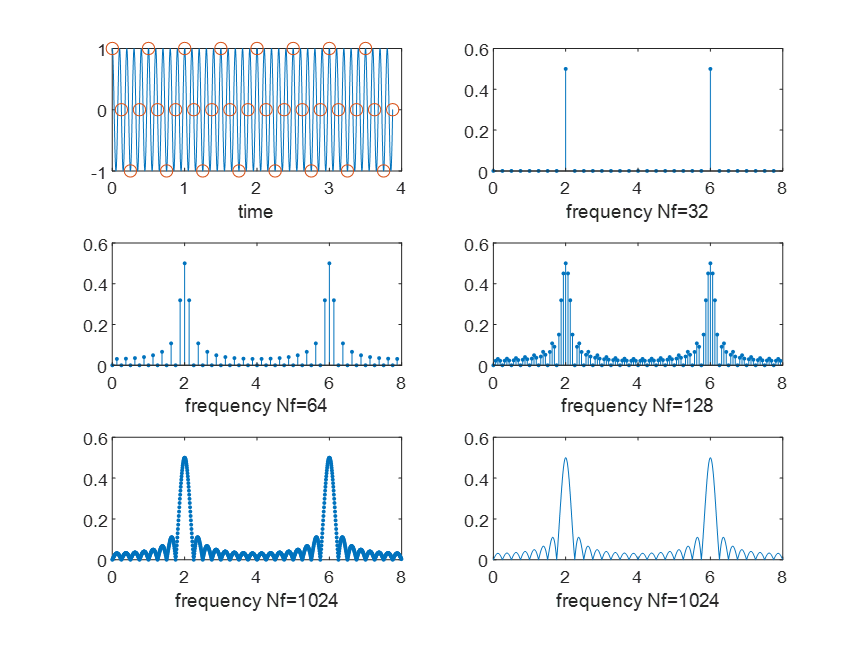
\includegraphics[width=1\linewidth]{运行结果.png}
    \caption{运行结果}
    \label{fig:result}
\end{figure}

\subsection{Question and Explaination}
\vspace{1em}

(0). About a real cosine signal that the theorem of Shannon is satisfied.

假设一段用DFT评估后的余弦信号,采样后会出现两个波峰,一个为7Hz,一个为1Hz的原因是:当采样频率大于2倍信号频率(即大于2f₀)时,根据奈奎斯特采样定理,信号可以被无失真地重建,频谱中不会出现混叠现象,信号的频率分量会在频谱中准确地呈现出来。当信号频率为1Hz,采样频率为8Hz时,由于1Hz低于奈奎斯特频率4Hz,频谱中只会出现1Hz处的峰值。而当信号频率为7Hz时,7Hz高于奈奎斯特频率4Hz,会发生混叠,混叠后的频率为1Hz,同时由于实信号的频谱对称性,频谱中会出现1Hz和7Hz两个主要的频率分量。
下文问题均以上面叙述为基础展开分析。
\vspace{3em}


(1). What is the minimum sampling frequency such that there is no aliasing?

为了避免混叠,最小采样频率应满足奈奎斯特定理,即采样频率至少要是信号最大频率的两倍。实验中的\(f_0=1Hz\),所以\(f_{smin}=2f_0=2Hz\)。
\vspace{3em}

(2). This signal is sampled with a sampling frequency equal to 8Hz. The number of samples \(N_t\) is fixed at 32. An FFT(DFT) is performed with the number of frequency points \(N_f\) equal to 32, 64, 128, 1024. View the sampled signal and the module of signal spectrum. What do you see? Carefully analyze and explain all the observed phenomena.
\begin{enumerate}
    \item 生成了一个1Hz的余弦波,采样点均匀分布在0到4秒之间,能清晰看到信号的周期性。
    \item 频谱在1Hz处有一个明显的主峰,其他频率点值接近0,准确反映了信号频率。
     随着FFT点数增加,频率分辨率提高,主峰周围的谱线越来越平滑,但主峰幅度不变。
    \item 频谱通过归一化处理,消除了采样点数的影响,便于直接观察信号的频率成分。
    \item 由于信号频率是采样频率的整数倍,且FFT点数足够,所以避免了明显的频率泄露。
\end{enumerate}

\vspace{3em}

(3). What is the main lobe bandwidth you observed? Is it dependent on the number of FFT points?\vspace{1em}

随着FFT点数从32增加到1024,主瓣带宽从0.25 Hz逐渐减小到0.0078125 Hz。
当FFT点数增加时,主瓣带宽会变窄。这是因为FFT点数越多,频率辨率越高,频谱的细节呈现得越清晰。
\vspace{3em}

(4). Set the sampling frequency $f\_s$ to 8Hz, the number of samples $N\_t$ to 32, and the number of DFT points $N\_f$ to 32. Draw the figures of the modulus of the sinusoidal signal spectrum in the case where the signal frequency is equal to 3Hz. Why the two maximum values are 3Hz and 5Hz?

因为DFT具有频谱对称性,对于实信号,其频谱在正负频率处是对称的。根据公式
\begin{equation}
f_s - f_0 = 8Hz - 3Hz = 5Hz
\end{equation}
, 而由于采样频率为8Hz,负频率-3Hz会被映射到正频率区域,即8Hz-3Hz=5Hz处,形成另一个峰值。因此,频谱图中会出现两个最大值,分别位于3Hz和5Hz。
\vspace{3em}

(5). Draw the figures of the modulus of the sinusoidal signal spectrum in the case where the signal frequency is equal to 5Hz. Why the two maximum values are 3Hz and 5Hz?
\vspace{1em}

根据奈奎斯特采样定理,信号频率超过4Hz时会产生混叠,混叠到3Hz。同时由于实信号频谱的对称性,5Hz的原始频率和3Hz的混叠频率在频谱中对称出现,形成两个峰值。
\vspace{3em}

(6). Draw the figures of the modulus of the sinusoidal signal spectrum in the case where the signal frequency is equal to 10Hz. Why the two maximum values are 2Hz and 6Hz?\vspace{1em}

根据奈奎斯特采样定理,10Hz>4Hz,混叠后映射到2Hz。同时,由于实信号频谱的对称性,除了2Hz外,还会有对称的峰值出现在6Hz(8Hz-2Hz)。因此,频谱模量图形中会出现两个最大值,分别位于2Hz和6Hz。\vspace{3em}


\section{Conclusion}
奈奎斯特定理的验证:
实验证实了奈奎斯特定理,即采样频率必须至少是信号最高频率的两倍,以避免混叠。


FFT点数的影响:
随着FFT点数从32增加到1024,频率分辨率显著提高。观察到的主瓣带宽从0.25 Hz逐渐减小到0.0078125 Hz。这表明,增加FFT点数可以更精确地呈现信号的频率成分,使频谱的细节更加清晰。


频谱泄漏与窗函数:
实验表明,当信号频率是采样频率除以样本数 Nt的整数倍,并且FFT点数 Nf足够多时,频谱泄漏被最小化。这在频谱中表现为尖锐且清晰的主峰。

本课程着重教授了matlab的高效使用,使用一些经典的非参数频率估计方法,了解了典型的参数化高分辨率的方法,最终掌握了使用matlab对一些光谱频率分析技术的编程,受益匪浅。



\end{document}